\section{Introduction}

\subsection{Context and justification}

The Musashi-1 (MSI-1) protein belongs to a family of neural RNA-binding proteins (RBPs) that play a fundamental role in neural development in both vertebrates and invertebrates \cite{nakamura_1994,sakakibara_1996, good_1998, imai_2001}. In particular, the mouse MSI-1 consists of 362 aminoacids with a molecular mass of 39 kDa \cite{sakakibara_1996}, and contains 2 sequences of around 80 to 90 aminoacids that interact with RNA (RRMs; short for RNA-recognition motifs) following the consensus sequence \texttt{RU}$_n$\texttt{AGU}\footnote{Following the IUPAC standard for degenerate base symbols, \texttt{R} represents both an Adenine (\texttt{A}) and a Guanine (\texttt{G}). Refer to \cite{cornish_1985} for the complete IUPAC standard.}$^,$\footnote{\texttt{U}$_n$ stands for repeating \texttt{U} within the consensus sequence $n$ times. In most cases, $n\in\left\{1,2,3\right\}$ \cite{imai_2001}.} \cite{imai_2001,zearfoss_2014}.\\

Despite multiple efforts, the complete structure of any of the MSI-1 protein homologues remains a mystery. The most notable successes have only been able to completely elucidate MSI-1's RRM1 and RRM2 domains \cite{nagata_1999,miyanoiri_2003,ohyama_2011,lan_2019}, see for example \textbf{Figure \ref{fig:3DRRM1}} for the 3D structure of RRM1. 

\begin{figure}[htbp!]
    \centering
    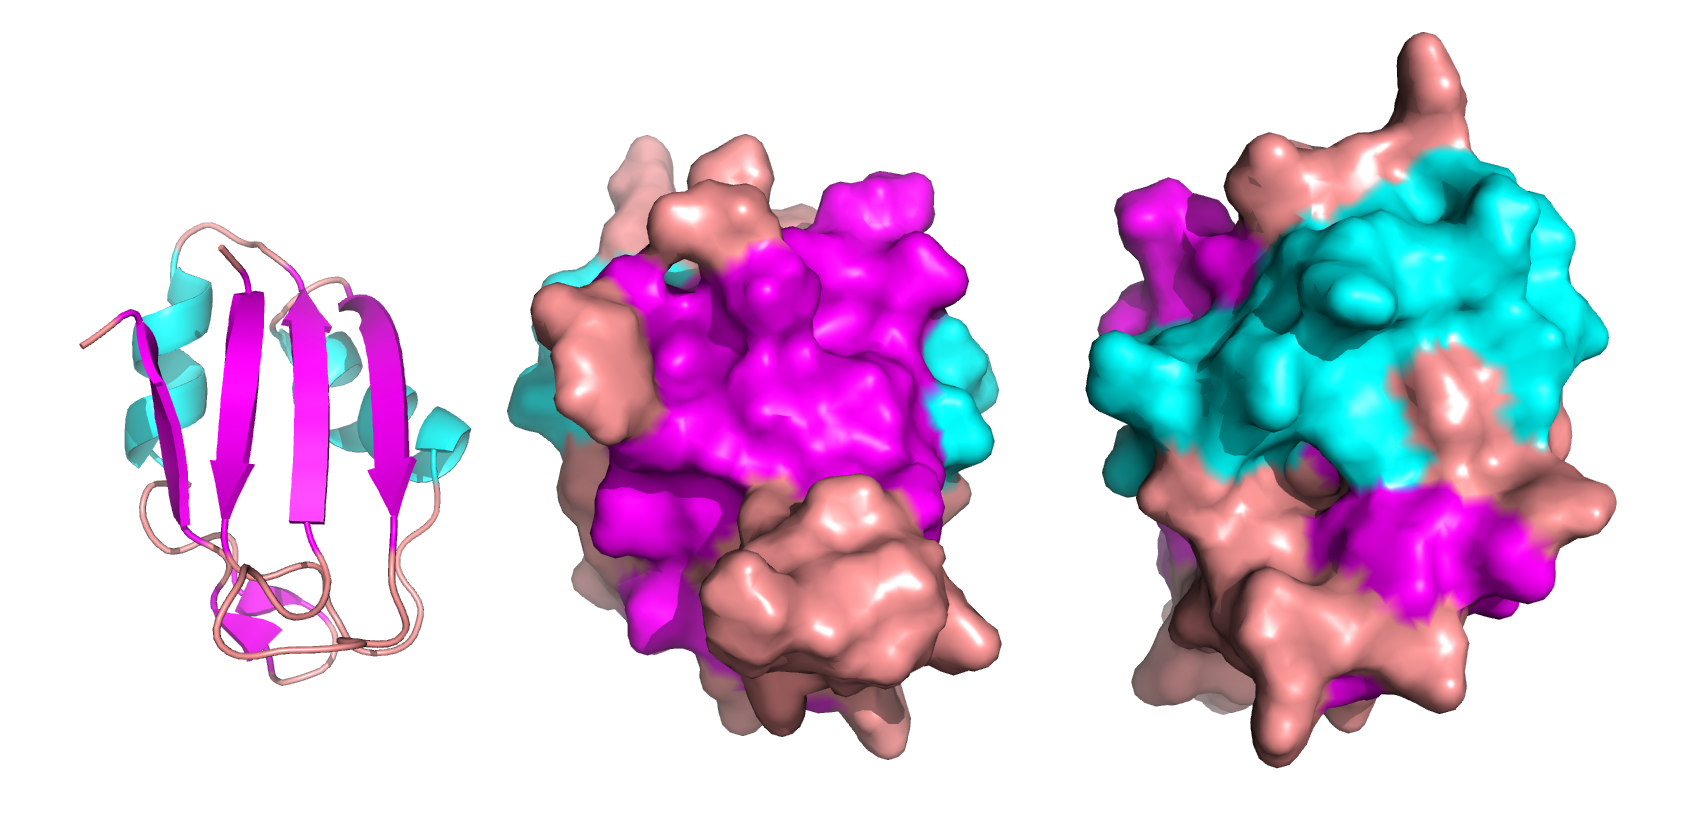
\includegraphics[width=0.9\linewidth]{assets/RRM1_various.png}
    \caption[3D RRM1 structure of the MSI-1 protein constructred by means of protein crystalization and RMN.]{3D RRM1 structure of the MSI-1 protein constructred by means of protein crystalization and RMN. From left to right: RRM1 in \textit{cartoon} setting, RRM1 in \textit{surface} setting and RRM1 in \textit{surface} setting turned 180$^\circ$. Colors represent the secondary structures found within the protein: cyan corresponds to $\alpha$-helices, magenta corresponds to $\beta$-sheets and salmon corresponds to \textit{random coil}. The model was retrieved from \href{https://www.uniprot.org/uniprotkb/Q61474/entry}{\texttt{Uniprot} entry \texttt{Q61474}}. Visualized through \href{https://pymol.org/2/}{\texttt{Pymol}}.}
    \label{fig:3DRRM1}
\end{figure}

\pagebreak

At the moment, the available complete MSI-1 structures only originate from computational predictions, such as the one shown in \textbf{Figure \ref{fig:3DMSI}} which is an aminoacid-sequence-based prediction yielded by \href{https://alphafold.ebi.ac.uk/}{\texttt{AlphaFold}} \cite{jumper_2021}.

\begin{figure}[htbp!]
    \centering
    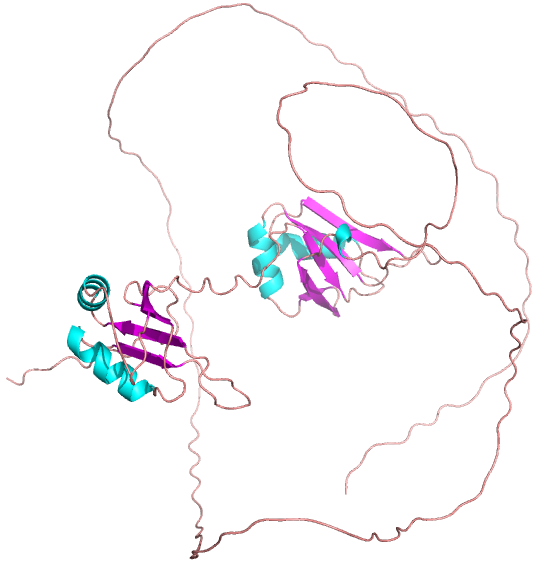
\includegraphics[width=0.5\linewidth]{assets/MSI1_complete.png}
    \caption[3D mouse MSI-1 structure as predicted by \texttt{AlphaFold}.]{3D mouse MSI-1 structure as predicted by \href{https://alphafold.ebi.ac.uk/}{\texttt{AlphaFold}}, in \textit{cartoon} setting. Colors represent the secondary structures found within the protein: cyan corresponds to $\alpha$-helices, magenta corresponds to $\beta$-sheets and salmon corresponds to \textit{random coil}. The model was retrieved from \href{https://www.uniprot.org/uniprotkb/Q61474/entry}{\texttt{Uniprot} entry \texttt{Q61474}}. Visualized through \href{https://pymol.org/2/}{\texttt{Pymol}}.}
    \label{fig:3DMSI} 
\end{figure}

With the surge of synthetic biology during the past two decades, RBPs such as MSI-1 have gained a special interest for their applicability as post-transcriptional regulators of gene expression in synthetic gene circuits \cite{belmont_2010,cao_2015,katz_2019}. In particular, Dolcemascolo and colleagues pioneered by designing a synthetic genetic circuit employing MSI-1 as post-transcriptional regulator \cite{dolcemascolo_2022}. In addition, they also exploited MSI-1's particularity of binding to fatty acids in addition to RNA, out of which the cis-9-Octadecenoic acid (also known as oleic acid) presents a higher binding affinity. The latter interaction weakens the MSI-1 protein's RNA-binding affinity, resulting in a dissociation between MSI-1 and the RNA sequence \cite{dolcemascolo_2022,clingman_2014}. In fact, the pocket in which the fatty acids interact with the RMM1 domain of MSI1 can be easily seen in the rightmost protein in \textbf{Figure \ref{fig:3DRRM1}}.\\

Therefore, in order to confidently add MSI-1 as an allosteric regulator to the synthetic biologist's toolbox, there is a need to understand how the underlying interaction mechanisms work. Clingman and colleagues are were the first who performed docking simulations with the MSI-1 core RNA-binding-motif and several fatty acids \cite{clingman_2014}. Nevertheless, these results only hold for the aforementioned RNA-motif: it is expected that any mutation on the RNA-motif would drastically impact the manner in which MSI-1 interacts with the RNA.

\subsection{Objectives}

This Master's Thesis aims to extend the knowledge behind the allosteric interactions occurring in the MSI-1 proteins by performing docking simulations between MSI-1's RRM1 domain, several RNA motifs and fatty acids, with the objective of obtaining a model for each of the combinatorial cases.\\

This general objective breaks down into the following specific objectives:

\begin{enumerate}
    \item \textit{In silico} Generate the 3D structures of 5 mutant MSI-1 RNA-binding motifs used in \cite{dolcemascolo_2022}. The 3D structures of the motifs will depend on the sequence-based-prediction of their secondary structures.
    \item Assess the structure of MSI-1's RRM1-RNA mutant complex through docking for each of the mutants.
    \item Assess the structure of MSI-1's RRM1-fatty acid complex through docking for each of the fatty acids of interest: oleic acid, linoleic acid, palmitoleic acid, arachidonic acid and stearic acid.
    \item Keep the top 2 fatty acids whose interaction with MSI-1 is the clearest.
    \item Assess the structure of RNA mutant-MSI-1's RRM1-fatty acid complex through the coupling of the docking models obtained.
\end{enumerate}
    
\subsection{Impact on sustainability, social-ethical and diversity}

\subsubsection{Sustainability}

The result of this Master's Thesis has had a negligible but negative impact on sustainability. This impact originates on the energy consumption during the following steps:

\begin{enumerate}
    \item Design and debugging of the docking pipeline followed in this work.
    \item Computation of the different models.
\end{enumerate}

This impact can be considered negligible because the net amount of energy consumed during the computations is very small. Nevertheless, it is important to highlight this aspect as there is room for improvement: the source code of the docking software employed in this work is mainly composed of two programming languages: \texttt{C} (72\%) and \texttt{Python} (28\%).\\

Pereira and colleagues developed a benchmark to order programming\linebreak languages with respect of their energy consumption when executing well-known computer science algorithms and data structures \cite{pereira_2017}. Their finding was that the least energy consuming programming language was \texttt{C}, while \texttt{Python} was one of the most energy consuming.\\

It can be discussed that, in order to reach minimal energy consumption, the programming language to be used in software that is going to be distributed and executed multiple times should be exclusively \texttt{C}. The disadvantages of \texttt{C} are that it takes more time to write a full program than with higher level languages (such as \texttt{Python}), it is more difficult to mantain a codebase written in \texttt{C} and that \texttt{C} is not a particularly accessible programming language for non-computer scientists.\\

There is a trade-off that has be to be considered. Let $L$ be a programming language, $E_{W_L}$ be the energy consumed by a computer during the crafting of a software written in $L$, $E_{E_L}$ be the energy consumed by a computer during one execution of the software written in $L$ (in this particular case, one docking simulation with some fixed parameters) and $n$ be the number of times the software is executed, then it is possible to approximate $E_{T_L}(n)$ (the total energy consumed by the software written in $L$ at the moment $n$) as follows:

\begin{equation}
    \label{eq:power}
    E_{T_L}(n)\approx E_{W_L} + n\times E_{E_L}         
\end{equation}

For the pair \texttt{Python} and \texttt{C}, we have that $E_{W_\text{\texttt{Python}}} <<< E_{W_\text{\texttt{C}}}$ and $E_{E_\text{\texttt{Python}}} >>> E_{E_\text{\texttt{C}}}$. So the larger $n$ becomes (the number of times the software is executed), by \textbf{Equation \ref{eq:power}}, \texttt{Python} becomes less and less energy efficient when compared to \texttt{C}.\\

Nevertheless, as mentioned previously, the codebase of the software used is in its majority written in \texttt{C}, the energy consumption of a personal computer is low and the number of executions $n$ in this work is small (less than $10^2$). Therefore this negative impact on energy consumption can be considered negligible.

\subsubsection{Social and ethical responsibility}

The technical nature of this work separates it from any positive nor negative impacts on socio-ethical aspects. There are no conflicts of interests with the results, and this work's material (models and source codes) are freely available to anyone through a public \texttt{GitHub} repository.\\

In addition, this work doesn't have any socio-ethical motivations, as the main objective is to gather more technical knowledge for the field of molecular biology.


\subsubsection{Diversity, gender and human rights}

Again, the technical nature of this work separates it from any positive nor negative impacts on diversity, gender and human rights. The references and materials employed within this work were used without any gender nor race bias.\\

Furhermore, this work doesn't have any diversity, gender nor human rights motivations. However, this work attempts to be accessible to as many people as possible, in the spirit of the universal right for knowledge and education. Moreover, this work exclusively employed license-free and open sourced software so that all the dependencies are accessible to anyone.

\subsection{Approach and methods}

This work aims to extend the work of Dolcemascolo and colleagues \cite{dolcemascolo_2022} where they designed a synthetic genetic circuit that employed MSI-1 as post-\linebreak transcriptional regulator. Thanks to the plasticity of RNA, several mutants of MSI-1's RNA-binding core motif were designed, and it was shown that gene regulation (which is tightly dependent on the MSI-1-RNA interaction) was altered for all mutants: some of them displayed an increase in regulation fold change while others displayed a decrease. In addition, the effects of MSI-1 induced regulation were partially nullified in presence of oleic acid.\\

The initial step of this work will consist in the retrieval of several 3D structures from the appropriate databases:

\begin{itemize}
    \item the 3D structure of mouse MSI-1's RMM1 is retrieved from \href{https://www.uniprot.org/}{\texttt{UniProt}}.
    \item the 3D structures of several fatty acids (oleic acid among them) are retrieved from \href{https://www.chemspider.com/}{\texttt{chemspider}}.
\end{itemize}

Next, some of the RNA sequences employed in \cite{dolcemascolo_2022} are retrieved and their 3D model structures are computed by means of \href{https://nupack.org/}{\texttt{NUPACK}} and \href{https://rnacomposer.cs.put.poznan.pl/}{\texttt{RNAComposer}} web server.\\

Then, all the docking simulations are performed:

\begin{enumerate}
    \item Between each RNA sequence and MSI-1 RMM1.
    \item Between each fatty acid and MSI-1 RMM1.
\end{enumerate}

The choice of docking software will vary for the type of docking simulation to be performed:

\begin{itemize}
    \item For protein-RNA docking, the docking software will be \href{https://lightdock.org/}{\texttt{LightDock}} because it is license-free, open source and it is partially written in \texttt{Python}.
    \item For protein-lipid docking, the docking software will be \href{https://vina.scripps.edu}{\texttt{AutoDock Vina}}, aided by \href{https://ccsb.scripps.edu/mgltools/}{\texttt{AutoDock Tools}} for the preparation step.
\end{itemize}

 The best models will be selected based on the chosen scoring function and biological significancy. In addition, all the models will be visualized with \href{https://pymol.org/2/}{\texttt{Pymol}}.

\subsection{Work plan}

This work is divided in the following tasks (and respective subtasks):

\begin{enumerate}
    \item Perform docking simulations of MSI-1 and a collection of mutants of the MSI-1 RNA-binding-motif.
        \begin{enumerate}
            \item Generate in silico a collection of up to 5 interesting mutant MSI-1 RNA-binding motifs.
            \item Perform docking simulations between MSI-1 and each of the mutants.
            \item Discard those mutants whose interaction with MSI-1 is poor.
        \end{enumerate}
    \item Perform docking simulations of MSI-1 and a collection of fatty acids.
        \begin{enumerate}
            \item Perform docking simulations between MSI-1 and several fatty acids of interest: oleic acid, linoleic acid, palmitoleic acid, arachidonic acid and stearic acid.
            \item Keep the top 2 fatty acids whose resulting model is the best.
        \end{enumerate}
    \item Perform docking simulations of MSI-1 and a subset of mutants of the MSI-1 RNA-binding-motifs in presence of fatty acids.
    \item Coupling of the successful docking models to visualize the lipid-MSI1-RNA complex.
    \pagebreak
    \item Defense preparation
        \begin{enumerate}
            \item Manuscript
            \item Presentation
        \end{enumerate}
\end{enumerate}

The landmarks of this work are distributed among the following continuous assessment tests:

\begin{itemize}
    \item Continuous Assessment Test 1: Thesis Definition and Work Plan.
    \item Continuous Assessment Test 2: Work Development (Phase 1).\\
        Landmarks:
        \begin{itemize}
            \item Generate in silico a collection of up to 5 interesting mutant MSI-1 RNA-binding motifs.
            \item Perform docking simulations between MSI-1 and each of the mutants {\color{red}\textit{(partially)}}.
        \end{itemize}
    \item Continuous Assessment Test 3: Work Development (Phase 2).
        \begin{itemize}
            \item Perform docking simulations between MSI-1 and each of the mutants.
            \item Discard those mutants whose interaction with MSI-1 is poor.
            \item Perform docking simulations between MSI-1 and several fatty acids of interest: oleic acid, linoleic acid, palmitoleic acid, arachidonic acid and stearic acid {\color{red}\textit{(partially)}}.
        \end{itemize}
    \item Continuous Assessment Test 4: Thesis Closure and Presentation.
        \begin{itemize}
            \item Perform docking simulations between MSI-1 and several fatty acids of interest: oleic acid, linoleic acid, palmitoleic acid, arachidonic acid and stearic acid.
            \item Keep the top 2 fatty acids whose resulting model is the best.
            \item Manuscript closure.
            \item Presentation closure.
        \end{itemize}
\end{itemize}

\pagebreak

The work plan is summarized in \textbf{Figure \ref{fig:gnatt}}:

\begin{figure}[htbp!]
    \centering
    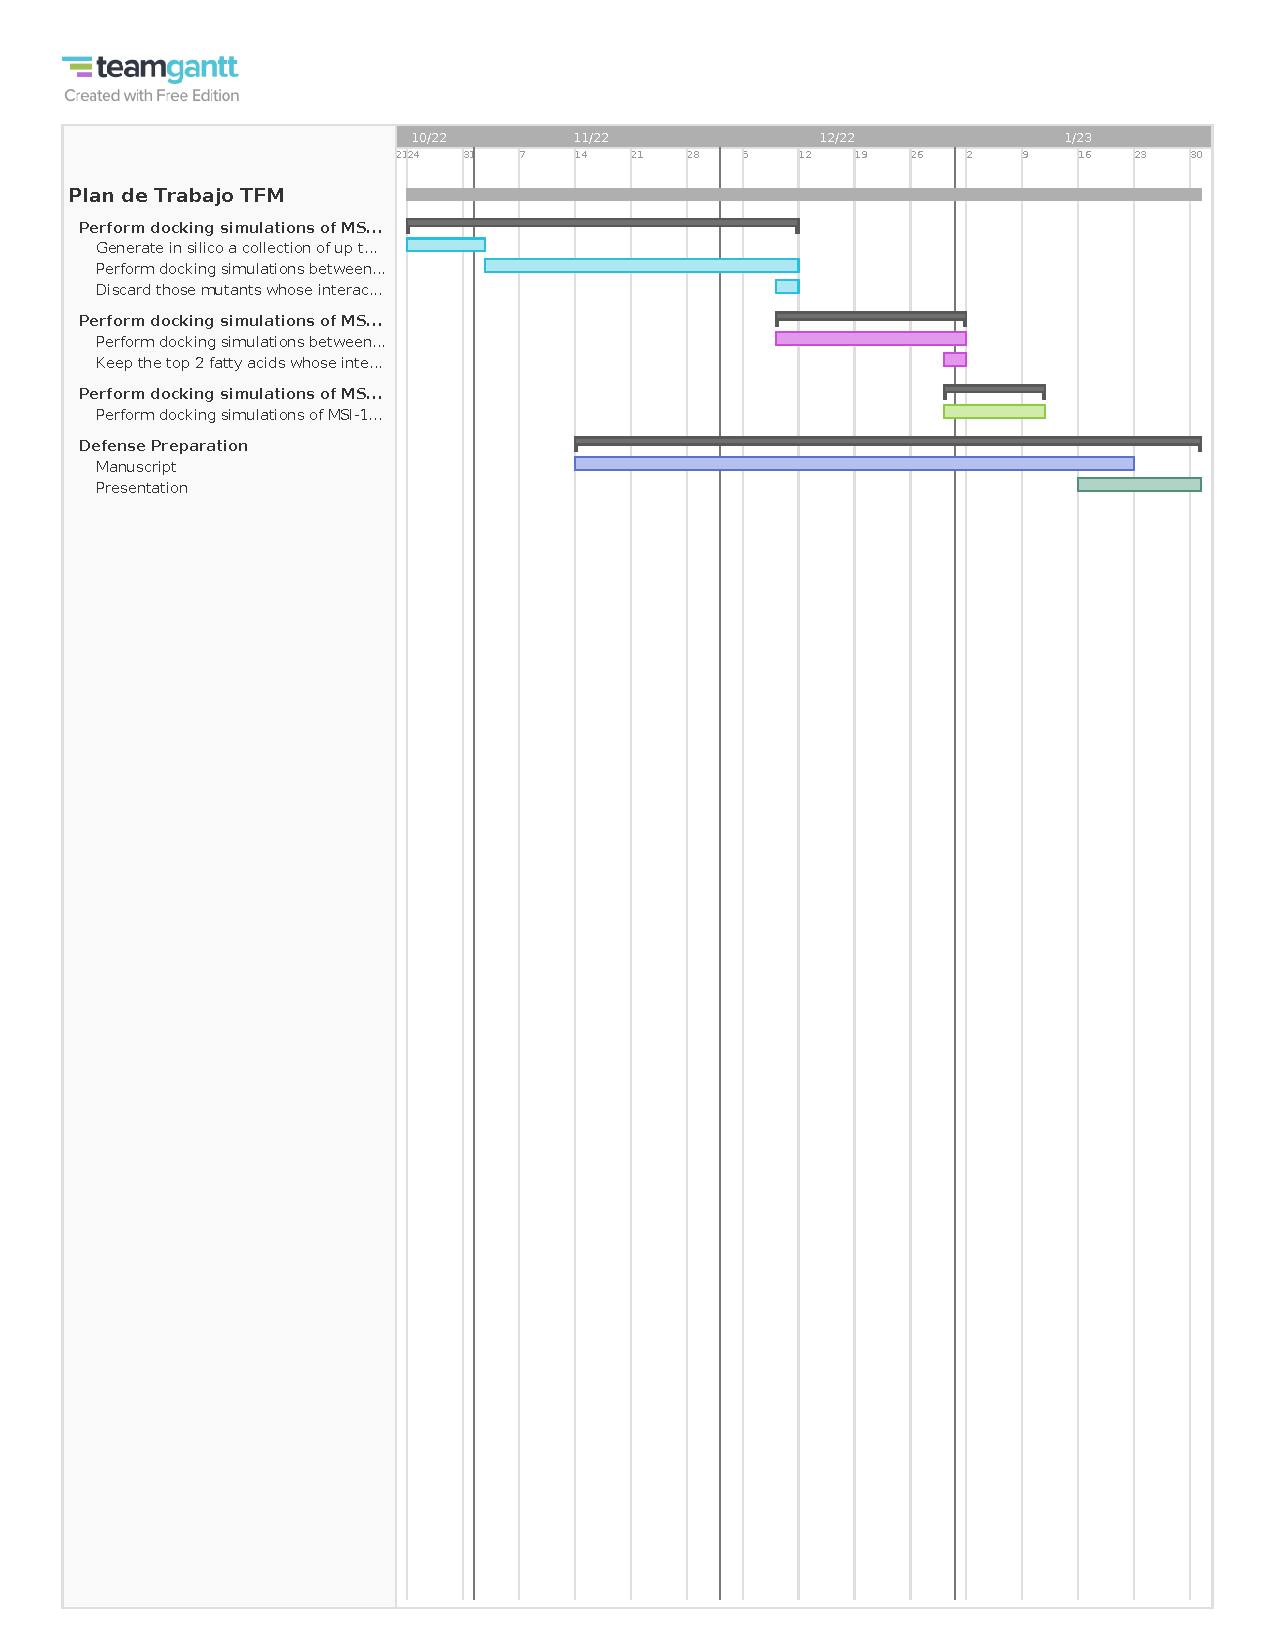
\includegraphics[width=\linewidth, trim={1cm 18.5cm 1cm 2cm},clip]{assets/Plan_de_Trabajo_TFM.pdf}
    \caption{Work plan summarized in a Gnatt chart.}
    \label{fig:gnatt}    
\end{figure}

\subsection{Summary of obtained products}

The main products of this work are:

\begin{enumerate}
    \item The current Master's Thesis manuscript.
    \item 3D structures of 5 MSI-1 RNA-motifs used in \cite{dolcemascolo_2022}.
    \item A series of \texttt{Python} and \texttt{Bash} scripts used to execute the docking pipeline.
    \item A total of 50 protein-RNA docking models (10 for each RNA-motif).
    \item A total of 45 protein-lipid docking models (9 for each fatty acid).
    \item\href{https://lightdock.org/tutorials/0.9.3/rna_docking}{A step-by-step tutorial on how to perform a simple protein-RNA docking with \texttt{LightDock}}.
\end{enumerate}

Resulting products are available in different repositories:
\begin{enumerate}
    \item The direct products of this work are present in \href{https://github.com/luksgrin/UOC_TFM}{this \texttt{GitHub} repository}.
    \item The step-by-step tutorial on how to perform a simple protein-RNA docking with \texttt{LightDock} is available at \href{https://github.com/lightdock/lightdock.github.io}{the \texttt{LightDock} \texttt{GitHub} repository}, and on the \href{https://lightdock.org/tutorials/}{\texttt{LightDock} tutorials page}.
\end{enumerate}

\subsection{Summary of other sections of this report}

% Breve explicación de los contenidos de cada capítulo y su relación con el proyecto global. 

The remaing sections of this manuscript are:

\begin{itemize}
    \item\textbf{State of the art}\\
        Introduction to Synthetic biology, RNA-binding proteins and the Musashi-1 RNA-binding protein family.
    \item\textbf{Materials and methods}\\
        Detailed description of the procedure followed within this work
    \item\textbf{Results}\\
        Main findings, their biological meanings and showcasing of the obtained products.
    \item\textbf{Conclusions and further work}\\
        The findings obtained are discussed in context of this work's original objectives. Further work that can extend this Master's Thesis is described.
    \item\textbf{Glossary}
    \item\textbf{References}
    \item\textbf{Appendix}
\end{itemize}